\newthought{\textbf{Adinda Awaliah - 2020903430004 - TRKJ 3B}}

\newday{\textbf{1-2 desember 2022} - Instalasi dan Konfigurasi Apache Hadoop}
\begin{enumerate}
\item Kendala dan Solusi
\newline praktikum instalasi apache hadoop tidak ada kendala. konfigurasi apache hadoop terkendala pada saat perintah jps, hasil yang muncul hanya 2jps, solusinya kembali ke langkah ssh, dan untuk menampilkan jps harus berada pada /usr/local/hadoop/etc/hadoop

\item Kesimpulan
\newline berhasil melakukan instalasi. berhasil melakukan konfigurasi.

\begin{figure}[!ht]
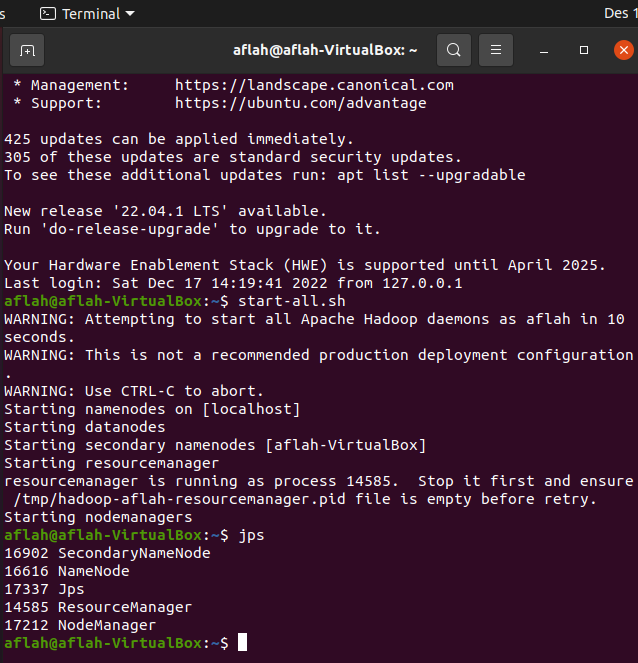
\includegraphics[width=\textwidth]{AdindaAwaliah/jps}
\caption{hasil dari jps}
\label{gam:jps}
\end{figure}

\begin{figure}
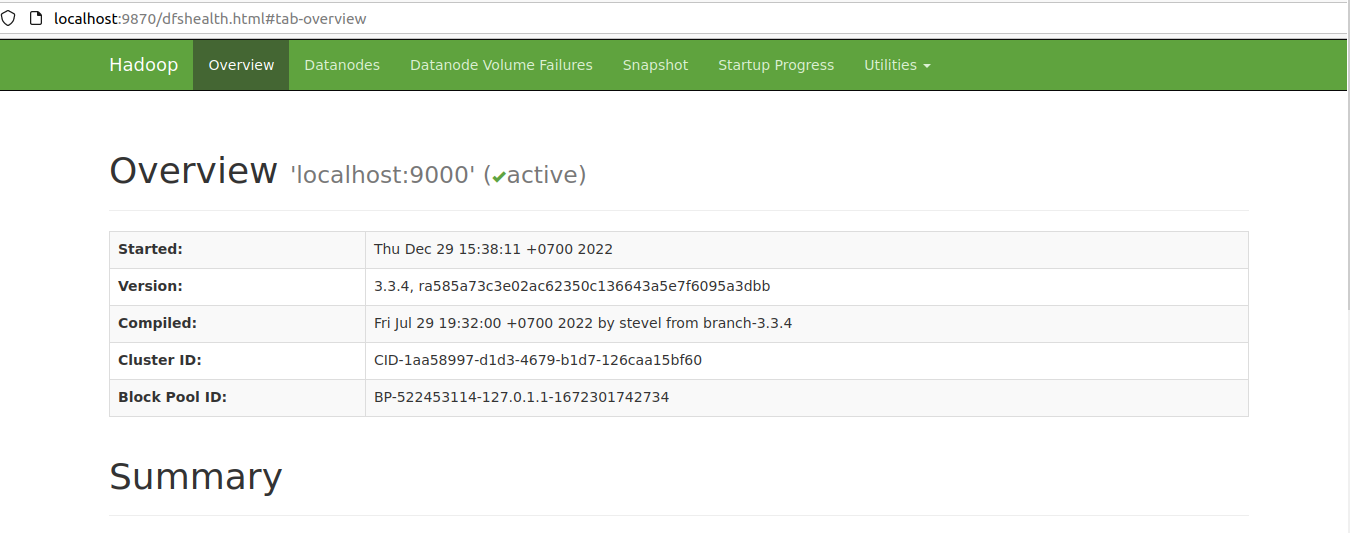
\includegraphics[width=\textwidth]{AdindaAwaliah/konfigurasi apache hadoop web 9870}
\caption{apache hadoop web 9870}
\label{gam:konfigurasi apache hadoop web 9870}
\end{figure}

\begin{figure}
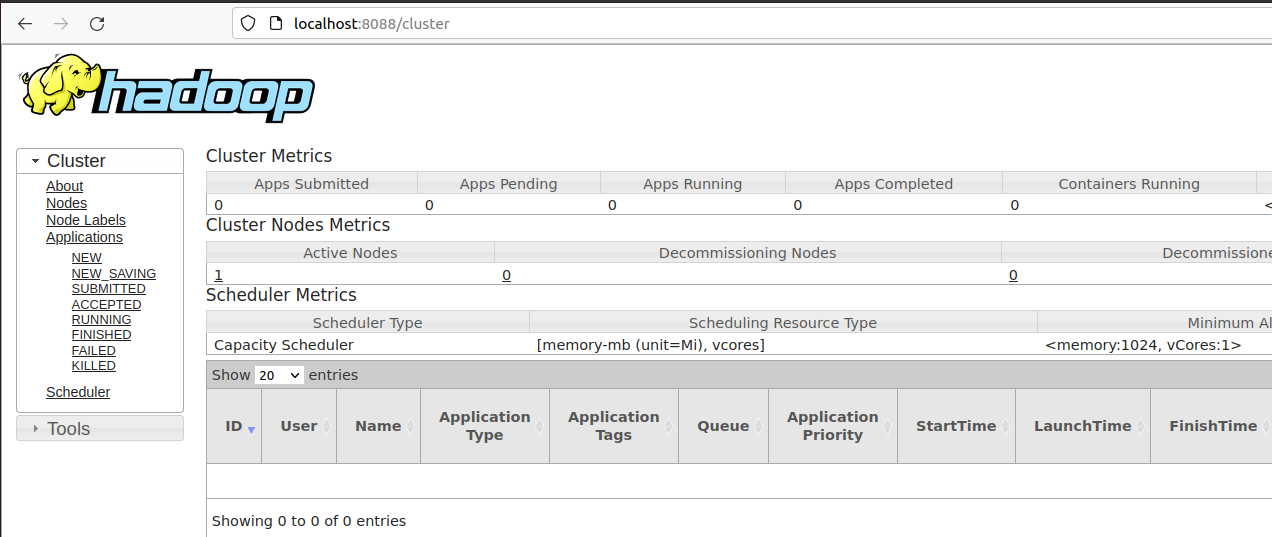
\includegraphics[width=\textwidth]{AdindaAwaliah/konfigurasi apache hadoop web 8088}
\caption{apache hadoop web 8088}
\label{gam:konfigurasi apache hadoop web 8088}
\end{figure}

\end{enumerate}

\newday{\textbf{ 8-9 desember 2022}}
\begin{enumerate}
\item Kendala dan Solusi
% jelaskan kendala dan penyebab yang dialami saat mengikuti praktikum serta solusi atau langkah-langkah yang telah dilakukan

\item Kesimpulan
% berikan kesimpulan dari praktikum yang telah dikerjkan
\newline lanjutan instalasi apache hadoop

\end{enumerate}


\newday{\textbf{15 desember 2022}}
\begin{enumerate}
\item Kendala dan Solusi
% jelaskan kendala dan penyebab yang dialami saat mengikuti praktikum serta solusi atau langkah-langkah yang telah dilakukan

\item Kesimpulan
% berikan kesimpulan dari praktikum yang telah dikerjkan

\end{enumerate}

\newday{\textbf{16 desember 2022}}
\begin{enumerate}
\item Kendala dan Solusi
% jelaskan kendala dan penyebab yang dialami saat mengikuti praktikum serta solusi atau langkah-langkah yang telah dilakukan

\item Kesimpulan
% berikan kesimpulan dari praktikum yang telah dikerjkan

\end{enumerate}

\newday{\textbf{22 desember 2022}}
\begin{enumerate}
\item Kendala dan Solusi
% jelaskan kendala dan penyebab yang dialami saat mengikuti praktikum serta solusi atau langkah-langkah yang telah dilakukan

\item Kesimpulan
% berikan kesimpulan dari praktikum yang telah dikerjkan

\end{enumerate}

\newday{\textbf{23 desember 2022}}
\begin{enumerate}
\item Kendala dan Solusi
% jelaskan kendala dan penyebab yang dialami saat mengikuti praktikum serta solusi atau langkah-langkah yang telah dilakukan

\item Kesimpulan
% berikan kesimpulan dari praktikum yang telah dikerjkan

\end{enumerate}
